%*******************************************************************************
% Example chapter file for books, Copyright A K Peters, Ltd.
%*******************************************************************************
\chapter{Depth of Field with Bokeh Rendering}{Charles de Rousiers and Matt Pettineo}
\label{BokehRendering}

%-------------------------------------------------------------------------------
\section{Introduction}

In order to increase realism and immersion, current games make frequent use of depth of field to simulate lenticular phenomena. Typical implementations use blur based approaches to simulate a camera’s circle of confusion out-of-focus parts of a scene. While such approaches give reasonable results, important features are still missing. In particular, real cameras produce a typical effect that photographers call bokeh (blur in Japanese) appearing at contrasted locations of the final image. Bokeh reveals itself as  bright blurry spots whose shape depends on the camera’s aperture (typically, a circle, a pentagon, or octagon). 

Current and upcoming DirectX11 engines (i.e. Cry engine, Unreal Engine, ...) have recently shown a particular interest for such effects as attested by their most recent demos. Still, it  remains an up-coming technology and precise implementation details are not available yet.

Explicitly drawing the aperture’s shape with quad rendering for every pixel would be rather inefficient. Instead, we propose an hybrid method, mixing previous blur based approaches with quad rendering. Our method selects high contrasted points, and for each of them, renders a quad with an aperture texture. In order to achieve high performance, we use both atomic counters, texture image for random memory access, and the glDrawElementsIndirect draw command for avoiding CPU / GPU synchronizations. This efficient OpenGL 4.2 implementation allows to draw thousands of aperture’s shape at high frame-rate and ensures the temporal coherency of the rendered bokeh.


Key insight : bokeh shape appears mostyl on highly constrasted point 

Topic
Why it is important
Things covers by this chapter

%-------------------------------------------------------------------------------
\section{Relative Work}\label{Derousiers:RelativeWork}

\subsection{Depth of field phenomenon}
Depth of field is an important effect to convey realism, especially in opened scenes.

\textbf{Integration} For every pixel, of the rendered image a integration has to be computed . explain integration


\textbf{Bokeh shape}explain why we get the bokeh shape

	\begin{figure}[htb]\centering
	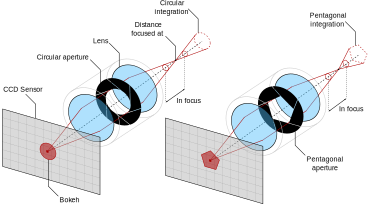
\includegraphics[width=\textwidth]{camera}
	\caption{Overview of the pipeline.}
	\label{YourName:fig1}
	\end{figure}


	\begin{figure}[htb]\centering
	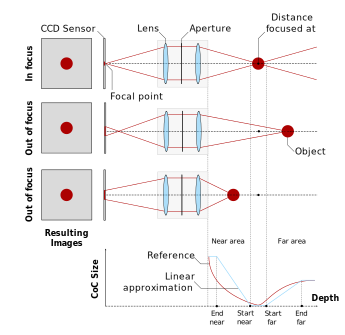
\includegraphics[width=\textwidth]{focus}
	\caption{Overview of the pipeline.}
	\label{YourName:fig1}
	\end{figure}


	\begin{figure}[htb]\centering
	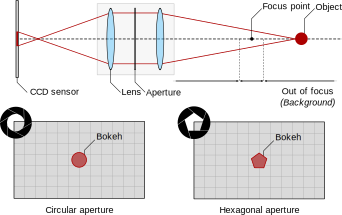
\includegraphics[width=\textwidth]{bokeh}
	\caption{Overview of the pipeline.}
	\label{YourName:fig1}
	\end{figure}

\begin{enumerate}
	\item The Technology Behind the DirectX 11 Unreal Engine "Samaritan" Demo, Martin Mittring, Bryan Dudash, GDC 2011
	\item Crysis 2 DX11 Ultra Upgrade, Tiago Sousa, Crytek, 2011
	\item $EXT_shader_image_load_store$, Jeff Bolz, Pat Brown, Barthold Lichtenbelt, Bill Licea-Kane, Eric Werness, Graham Sellers, Greg Roth, Nick Haemel, Pierre Boudier and Piers Daniell, 2010
	\item 3DMark11 Whitepaper, Furturemark, 2011
	\item Practical Post-Process Depth of Field, Earl Hammon, Jr. , Infinity Ward, GPU Gems 3
	\item Krivanev : Lot of overdraw
\end{enumerate}

	This chapter propose an OpenGL implementation proposed by Matt Pettineo~\cite{Pettineo11}

%-------------------------------------------------------------------------------
\section{Overview}
Presentation of the overall pipeline

	\begin{figure}[htb]\centering
	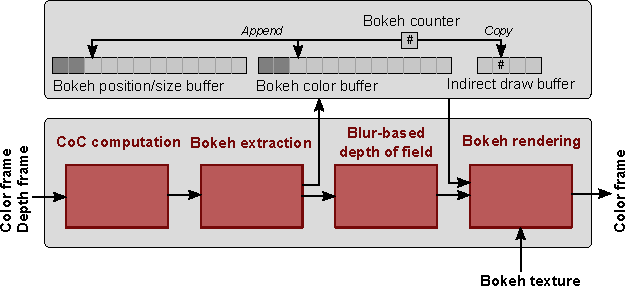
\includegraphics[width=\textwidth]{pipeline}
	\caption{Overview of the pipeline.}
	\label{YourName:fig1}
	\end{figure}

\subsection{Circles of confusion computation}
We compute the amount of blur 

\subsection{Bokeh detection}
Estimate
heuristic
atomic counter
append buffer

C/C++ application
\begin{lstlisting}[language=GLSL,float={htb},caption={Your caption.},label={YourName:listing1}]
in vec3 worldPosition;
in vec3 positionToLight;
out vec3 fragmentColor;

void main()
{
  // Calculate diffuse lighting
  vec3 toLight = normalize(positionToLight);
  vec3 normal = normalize(worldPosition);
  float diffuse = max(dot(toLight, normal), 0.0);
  fragmentColor = vec3(diffuse, diffuse, diffuse);
}
\end{lstlisting}

Fragment shader
\begin{lstlisting}[language=GLSL,float={htb},caption={Your caption.},label={YourName:listing1}]
in vec3 worldPosition;
in vec3 positionToLight;
out vec3 fragmentColor;

void main()
{
  // Calculate diffuse lighting
  vec3 toLight = normalize(positionToLight);
  vec3 normal = normalize(worldPosition);
  float diffuse = max(dot(toLight, normal), 0.0);
  fragmentColor = vec3(diffuse, diffuse, diffuse);
}
\end{lstlisting}


\subsection{Background blur effect}

\subsection{Foreground blur effect}

\subsection{Bokeh rendering}

C/C++ application
\begin{lstlisting}[language=GLSL,float={htb},caption={Your caption.},label={YourName:listing1}]
in vec3 worldPosition;
in vec3 positionToLight;
out vec3 fragmentColor;

void main()
{
  // Calculate diffuse lighting
  vec3 toLight = normalize(positionToLight);
  vec3 normal = normalize(worldPosition);
  float diffuse = max(dot(toLight, normal), 0.0);
  fragmentColor = vec3(diffuse, diffuse, diffuse);
}
\end{lstlisting}

Geometry shader
\begin{lstlisting}[language=GLSL,float={htb},caption={Your caption.},label={YourName:listing1}]
in vec3 worldPosition;
in vec3 positionToLight;
out vec3 fragmentColor;

void main()
{
  // Calculate diffuse lighting
  vec3 toLight = normalize(positionToLight);
  vec3 normal = normalize(worldPosition);
  float diffuse = max(dot(toLight, normal), 0.0);
  fragmentColor = vec3(diffuse, diffuse, diffuse);
}
\end{lstlisting}

instancing rendering
geometry shader expansion

%-------------------------------------------------------------------------------
\section{Results}

\subsection{Rendering}
	\begin{figure}[htb]\centering
	
\includegraphics[width=\textwidth]{todo}
	\caption{Rendering 1.}
	\label{YourName:fig1}
	\end{figure}

	\begin{figure}[htb]\centering
	
\includegraphics[width=\textwidth]{todo}
	\caption{Rendering 2.}
	\label{YourName:fig1}
	\end{figure}

\subsection{Performances}
	\begin{figure}[htb]\centering
	
\includegraphics[width=\textwidth]{todo}
	\caption{Performances.}
	\label{YourName:fig1}
	\end{figure}

%-------------------------------------------------------------------------------
\section{Discussion}
Temporal coherence and sub-pixel Aliasing
Pre-allocation of a large chunk of memory

%-------------------------------------------------------------------------------
\section{Conclusion}
Sum up

\textbf{Future work:} Several improvments would be done in order to improve performances. 
\begin{itemize}
	\item \textbf{Tile-version} : divide screen into four part and set one atomic-counter per part
	\item \textbf{Mipmap-rasterization} : rasterize bokeh at proper resolution (Approch done in 3DMark11)
\end{itemize}

%-------------------------------------------------------------------------------
\bibliographystyle{akpbib}
\bibliography{BokehRenderingBib}











